%%%%%%%%%%%%%%%%%%%%%%%%%%%%%%%%%%%%%%%%%%%%%%%%%%%%%%%%%%%%%%%%%%%%%%%%%%%

\documentclass{standalone}

\usepackage{amsmath}
\usepackage{mathptmx}
\usepackage{pgfplots}
\usetikzlibrary{external}
\tikzexternalize{frond-errors}
\pgfplotsset{compat=1.16}

%% IEEE uses Times Roman font, so we'll default to Times.
%% These three commands make up the entire times.sty package.
\renewcommand{\rmdefault}{ptm}
\renewcommand{\ttdefault}{pcr}
\normalfont\selectfont

\begin{document}

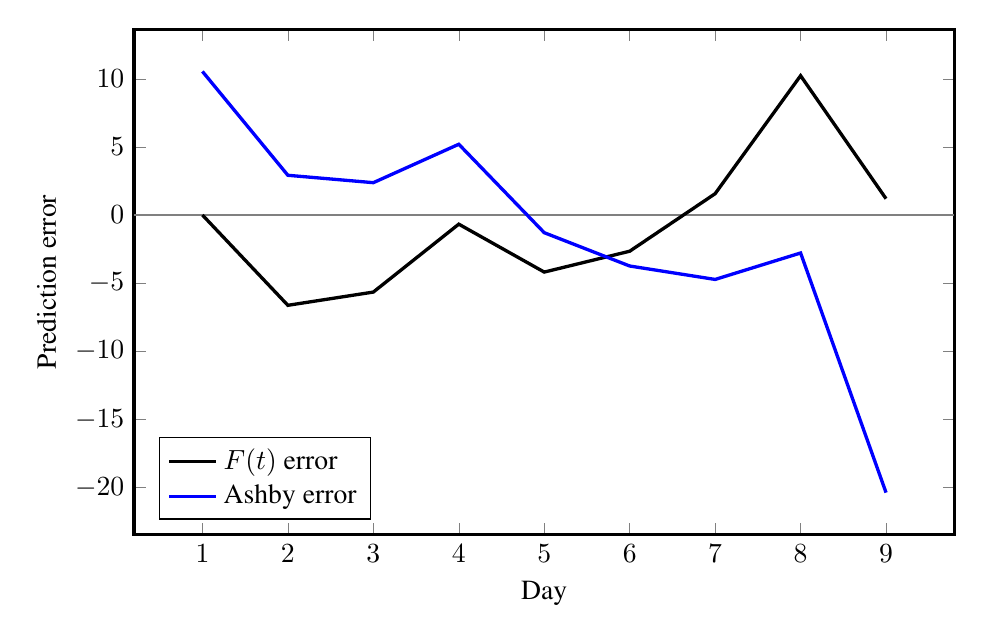
\begin{tikzpicture}
\tikzset{%%
  every mark/.append style={scale=1.0},%%
  scale=1.0%%
}
\pgfplotsset{%%
  every axis/.append style={font=\normalsize}%%
}
%%
\begin{axis}[%%
  axis line style=very thick,%%
  dotStyle/.style={very thick,mark=none},%%
  enlargelimits=true,%%
  height=8cm,%%
  legend cell align=left,%%
  legend pos=south west,%%
  width=12cm,%%
  %% x axis
  xlabel={\normalsize Day},%%
  %% y axis
  ylabel={\normalsize Prediction error},%%
  scaled y ticks=false,%%
  y tick label style=/pgf/number format/fixed%%
]
%%
%%
%% Horizontal line through origin.
\draw[gray,thin] ({rel axis cs:0,0}|-{axis cs:0,0}) -- ({rel axis cs:1,0}|-{axis cs:1,0});
%%
%%
%% Errors from using the formula with mean growth factor.
\addplot[dotStyle,black] coordinates {
  (1, 0)
  (2, -6.63000399999999)
  (3, -5.65829179572799)
  (4, -0.671367427406608)
  (5, -4.1900171953792)
  (6, -2.6588650082752)
  (7, 1.56573225822964)
  (8, 10.2297132174946)
  (9, 1.19756999857748)
};
\addlegendentry{$F(t)$ error}
%%
%%
%% Errors from using Ashby's equation.
\addplot[dotStyle,blue] coordinates {
  (1, 10.5417017781486)
  (2, 2.91718042678042)
  (3, 2.37476054097286)
  (4, 5.19639409191058)
  (5, -1.29778585412623)
  (6, -3.74429476572857)
  (7, -4.73042612023434)
  (8, -2.78758590846343)
  (9, -20.3837245179625)
};
\addlegendentry{Ashby error}
\end{axis}
\end{tikzpicture}

\end{document}
